\section{Finite Element Neutron Diffusion}
\label{sec:neutronDiffusion}

\begin{frame}{Finite Element Neutron Diffusion}
  \begin{itemize}
    \item Require neutron distribution to calculate power distribution, thermal
      feedback, eigenvalues, and other quantities of interest.
    \item Model reactor neutron distribution with the multigroup neutron
      diffusion equation.
    \item Solve multigroup neutron diffusion equation via Finite Element Method
      (FEM).
  \end{itemize}

  Begin with a set of energies $\{E_g\}$ for $g = 1,2,\ldots,G$ and arranged in
  order of decreasing energy by convention.
  \begin{equation}
    0 < E_G < E_{G-1} < \ldots < E_2 < E_1 < \nicesub{E}{max}
  \end{equation}
  Typically, for \mcc and fast reactors, $G=33$.
\end{frame}

\begin{frame}{Multigroup Neutron Diffusion Equation}
  In conventional notation, the multigroup neutron diffusion equation can be
  written as 
  \begin{equation}
    \label{eq:multigroup_diffusion}
    - \grad \cdot ( D_g(\vr) \grad \phi_g(\vr)) + \Sigma_{t,g}(\vr) \phi_g(\vr)= 
      \frac{\widetilde{\chi_g}(\vr)}{\keff} 
      \sum_{g'=1}^{G} \nu\Sigma_{f,g'}(\vr) 
      \phi_{g'}(\vr) + \sum_{g'=1}^{G} \Sigma_{s,g' \rightarrow g}(\vr) 
      \phi_{g'}(\vr)
  \end{equation}
  where 
  \begin{conditions} % custom environment designed for this purpose
    D_g(\vr)    & diffusion coefficient for energy group $g$ \units{cm}, \\
    \phi_g(\vr) & scalar neutron flux for energy group $g$
      \units{$\frac{1}{\text{cm}^2 \; \text{s}}$}, \\
    \Sigma_{t,g}(\vr) & macroscopic total cross-section for energy group $g$ 
      \units{$\frac{1}{\text{cm}}$}, \\
    \widetilde{\chi_g}(\vr) & effective fission spectrum for energy group $g$,\\
    \keff & effective neutron multiplication factor, \\
    \nu \Sigma_{f,g}(\vr) & 
      \parbox[t]{\columnwidth}{number of fission neutrons times microscopic 
        fission \\
        cross-section in energy group $g$ \units{$\frac{1}{\text{cm}}$}, }\\
    \Sigma_{s,g' \rightarrow g} (\vr) & 
      \parbox[t]{\columnwidth}{macroscopic scatter cross-section from
      energy group $g'$ to\\
      energy group $g$ \units{$\frac{1}{\text{cm}}$},} \\
    G & total number of energy groups%.
  \end{conditions}
\end{frame}

\begin{frame}{Removal Cross-Section}
  \begin{itemize}
    \item Rewrite by defining removal cross-section.
    \item Aids simplicity and numeric efficiency.
  \end{itemize}
  \begin{equation}
    \Sigma_{r,g}(\vr) = \Sigma_{t,g}(\vr) - \Sigma_{s,g \rightarrow g}(\vr)
  \end{equation}
  \begin{equation} 
    \label{eq:multigroup_removal}
    - \grad \cdot( D_g(\vr) \grad \phi_g(\vr)) + \Sigma_{r,g}(\vr) \phi_g(\vr) = 
      \frac{\widetilde{\chi_g}(\vr)}{\keff} 
      \sum_{g'=1}^{G} \nu\Sigma_{f,g'}(\vr) 
      \phi_{g'}(\vr) + \sum_{g'=1, g' \ne g}^{G} 
      \Sigma_{s,g' \rightarrow g}(\vr) \phi_{g'}(\vr)
  \end{equation}
\end{frame}

\begin{frame}{Combining Neutron Source}
  \begin{itemize}
    \item Neutron sources are combined into a single term.
    \item This will resemble the FEM formulation.
  \end{itemize}
  \begin{equation}
    \label{eq:multigroup_source}
    - \grad \cdot( D_g(\vr) \grad \phi_g(\vr)) + \Sigma_{r,g}(\vr) \phi_g(\vr) = 
      q_g(\vr)
  \end{equation}
  \begin{align}
    \label{eq:q}
    q_g(\vr) &= q_{fiss,g}(\vr) + q_{up,g}(\vr) + q_{down,g}(\vr) \\
    \label{eq:qfiss}
    q_{fiss,g}(\vr) &= \frac{\widetilde{\chi_g}(\vr)}{\keff} \sum_{g'=1}^{G} 
      \nu \Sigma_{f,g'}(\vr) \phi_{g'}(\vr), \\
    \label{eq:qup}
    q_{up,g}(\vr) &= \sum_{g'=g+1}^{G} \Sigma_{s,g' \rightarrow g}(\vr)
      \phi_{g'}(\vr), \\
    \label{eq:qdown}
    q_{down,g}(\vr) &= \sum_{g'=1}^{g-1} \Sigma_{s,g' \rightarrow g}(\vr)
      \phi_{g'}(\vr),
  \end{align}
\end{frame}

\begin{frame}{Collapsing $\chi$}
  \begin{itemize}
    \item It is necessary to describe effective fission spectrum
      $\widetilde{\chi}_g(\vr)$ in terms of isotopic $\chi_{i,g}$.
    \item This is done by preserving fission neutron production rate.
    \item Fission spectrum, $\chi$, is now unique to each finite element.
  \end{itemize}
  \begin{equation}
    \label{eq:chi_collapse}
    \widetilde{\chi_g}(\vr) = \frac{\sum_{i=1}^{N_I} \chi_{i,g}(\vr)
      \nu \Sigma_{f,i,g}(\vr) \phi_g(\vr)}
      {\sum_{i=1}^{N_I} \nu \Sigma_{f,i,g}(\vr) \phi_g(\vr)}
  \end{equation}
\end{frame}

\begin{frame}{Boundary Conditons}
  Consider a domain $\Omega$ with boundary $\partial \Omega$ and let $\nhat$ be
  the outward-normal unit vector.

  \begin{enumerate}
    \item Mirror. $\grad \phi_g(\vr) \cdot \nhat = 0 \; \forall \; 
      \vr \in \partial \Omega$.
    \item Albedo. $D_g(\vr) \grad \phi_g(\vr) \cdot \nhat + \albedo \phi_g(\vr)
      = 0 \; \forall \; \vr \in \partial \Omega$, where $\albedo$ is a constant
      specified by the user. For non-reentrant boundary condition, $\albedo =
      \half$. $\albedo = 0$ corresponds to mirror boundary condition and
      $\albedo \rightarrow \infty$ corresponds to Zero Flux boundary condition.
    \item Zero Flux. $\phi_g(\vr) = 0$ for $\vr \in \partial \Omega$.
  \end{enumerate}

  The order above corresponds to the order of boundary condition precedent with 
  the greater the integer, the greater the precedent.
\end{frame}

\begin{frame}{Finite Element Discretization}
  Divide the domain $\Omega$ into a set of unstructured finite elements 
  (e.g. Delaunay triangulation).
  \begin{equation}
    \label{eq:set_of_elements}
    \Omega = \Omega_1 \cup \Omega_2 \cup \Omega_3 \cup \ldots \cup
      \Omega_{N_E} 
  \end{equation}
  such that
  \begin{equation}
    \Omega = \{\Omega_e\} \; \text{for} \; e = 1,2,\ldots,N_E
  \end{equation}
  is a set of non-overlapping elements and
  \begin{equation}
    \Omega_i \cap \Omega_j = \emptyset.
  \end{equation}
\end{frame}

\begin{frame}{Finite Element Method}
  Multiply the multigroup neutron diffusion equation by a testing function
  $v(\vr) \in H_1(\Omega)$ and integrate over the problem domain. This yields
  the Weak Form of the problem.
  \begin{equation}
    \label{eq:fem_weak_form}
    - \int_{\Omega} \grad \cdot (D_g(\vr) \grad \phi_g(\vr)) v(\vr) \; d\vr
      + \int_{\Omega} \Sigma_{r,g}(\vr) \phi_g(\vr) v(\vr) \;d\vr=
      \int_{\Omega} q_g(\vr) v(\vr) \;d\vr
  \end{equation}
\end{frame}

\begin{frame}
  Allow the neutron source $q_g(\vr)$ to be constant over an element $\Omega_e$.
  Alternatively, a point source could be integrated numerically.
  \begin{align}
    q_g(\vr) &= q_{g,e} \; \forall \; \vr \in \Omega_e \\
    q_{g,e} &= q_{fiss,g,e} + q_{up,g,e} + q_{down,g,e} \\
    \label{eq:qelement_fiss}
    q_{fiss,g,e} &= \frac{\chi_{g,e}}{\keff} \sum_{g'=1}^G \nu
      \Sigma_{f,g',e} \phiavg_{g',e} \\
    \label{eq:qelement_up}
    q_{up,g,e} &= \sum_{g'=g+1}^G \Sigma_{s,g' \rightarrow g,e}
      \phiavg_{g',e}\\
    \label{eq:qelement_down}
    q_{down,g,e} &= \sum_{g'=1}^{g-1} \Sigma_{s,g' \rightarrow g,e}
      \phiavg_{g',e}\\
    \phiavg_{g,e} &= \frac{1}{N_p} \sum_{i \in \Omega_e}^{N_p} \phi_{i,g}
  \end{align}
  Additionally, allow all cross-sections to be constant within an element.
\end{frame}

\begin{frame}
  Separate the integration over the domain $\Omega$ into the summation of
  integrals over $\Omega_e$.
  \begin{equation} 
    \label{eq:element_by_element}
    -\sum_{e=1}^{N_E} D_{g,e} 
      \int_{\Omega_e} \grad \cdot \grad \phi_g(\vr) v(\vr) \; d\vr +
      \sum_{e=1}^{N_E} \Sigma_{r,g,e} \int_{\Omega_e} \phi_g(\vr) v(\vr) 
      \;d\vr = \sum_{e=1}^{N_E} q_{g,e} \int_{\Omega_e} v(\vr) 
      \; d\vr
  \end{equation}
  Use the Second Green's Theorem to rewrite the first integral
  \cite{textbookli}.
  %\footcite{textbookli}.
  \begin{multline} 
    -\sum_{e=1}^{N_E} D_{g,e} \int_{\partial \Omega_e} v(\vr) \grad
    \phi_g(\vr) \cdot \nhat \;ds + \sum_{e=1}^{N_E} 
      D_{g,e} \int_{\Omega_e} \grad \phi_g(\vr) \cdot \grad v(\vr) 
      \; d\vr + \\
      \sum_{e=1}^{N_E} \Sigma_{r,g,e} \int_{\Omega_e} \phi_g(\vr) v(\vr) 
     \; d\vr =
      \sum_{e=1}^{N_E} q_{g,e} \int_{\Omega_e} v(\vr) \; d\vr
  \end{multline}
\end{frame}

\begin{frame}
  \begin{itemize}
    \item Recognize the form of the boundary condition.
    \item Note that mirror and zero-flux boundary conditions can both be written
      as albedo boundary conditions.
  \end{itemize}
  \begin{multline}
    \label{eq:element_boundary}
    \sum_{e=1}^{N_E} \albedo \int_{\partial \Omega_e} v(\vr) 
      \phi_g(\vr) \;ds + \sum_{e=1}^{N_E} D_{g,e}
      \int_{\Omega_e} \grad \phi_g(\vr) \cdot \grad v(\vr) \; d\vr + \\
      \sum_{e=1}^{N_E} \Sigma_{r,g,e} \int_{\Omega_e} \phi_g(\vr) v(\vr) 
      \; d\vr =
      \sum_{e=1}^{N_E} q_{g,e} \int_{\Omega_e} v(\vr) \; d\vr
  \end{multline}
\end{frame}

\begin{frame}{Galerkin Finite Element Method}
  Galerkin Finite Element Method assumes the solution $\phi_g(\vr)$ is a linear
  combination of chosen basis functions $\{\basis_i\}$.
  \begin{equation} 
    \label{eq:linear_combination}
    \phi_g(\vr) = \sum_{i=1}^{DOF} \upsilon_{g,i} \, \basis_i(\vr)
  \end{equation}
  Coefficients $\{\upsilon_{g,i}\}$ will be solved in a linear system.
  $v(\vr)$ is arbitrary such that $v(\vr) \in H_1(\Omega)$ and is chosen to be a
  linear combination of the basis functions with unit magnitude.
  \begin{equation} 
    \label{eq:linear_superposition}
    v(\vr) = \sum_{j=1}^{DOF} \basis_j(\vr)
  \end{equation}
\end{frame}

\begin{frame}{Linear System of Equations}
  Including albedo form of boundary condition and assumption of linear
  combination of basis functions.
  \begin{multline}
    \label{eq:linear_equation}
    \sum_{i=1}^{DOF} \upsilon_{i,g} \sum_{j=1}^{DOF} \left(
      \sum_{e=1}^{N_E} \albedo \int_{\partial \Omega_e}
      \basis_i(\vr)  \basis_j(\vr) \;ds +
      \sum_{e=1}^{N_E} D_{g,e} 
      \int_{\Omega_e} \grad \basis_i(\vr) \cdot \grad \basis_j(\vr)\;d\vr
      \right.
      + \\
      \left.
      \sum_{e=1}^{N_E} \Sigma_{r,g,e}
      \int_{\Omega_e} \basis_i(\vr) \basis_j(\vr) \; d\vr \right) =
      \sum_{i=1}^{DOF} \left(
      \sum_{e=1}^{N_E} q_{g,e} 
      \int_{\Omega_e} \basis_i(\vr) \; d\vr \right)
  \end{multline}

  Rewriting in the form common to FEM.
  \begin{equation}
    \label{eq:fem_notation}
    a(\basis_i,\basis_j) = f(\basis_i)
  \end{equation}
  In the form common to linear systems.
  \begin{equation}
    \label{eq:matrix_notation}
    \ma \, \vu = \vf
  \end{equation}
  \[ \vu = \{\upsilon_{i,g}\} \]
\end{frame}

\begin{frame}{Properties of $\ma \, \vu = \vf$}
  Properties of the linear system include:
  \begin{itemize}
    \item Symmetric, positive-definite \cite{textbookhughes}.
    \item Solution, $\vu$, is unique and bounded by Lax-Milgram Lemma 
      \cite{textbookli}.
  \end{itemize}
  Solution via Conjugate Gradient (CG) method 
  \cite{Kelley1995IterativeEquations}.

  It is natural to populate the matrix $\ma$ in an element-by-element procedure.
  \begin{align}
    A_{i,j,g} &= \sum_{e=1}^{N_E} A_{i,j,g,e} \\
    f_{i,g} &=  \sum_{e=1}^{N_E} f_{i,g,e}
  \end{align}
\end{frame}

\begin{frame}{Triangular Elements}
  \begin{figure}
    \centering
    \subfloat[General Triangle Element.]
      {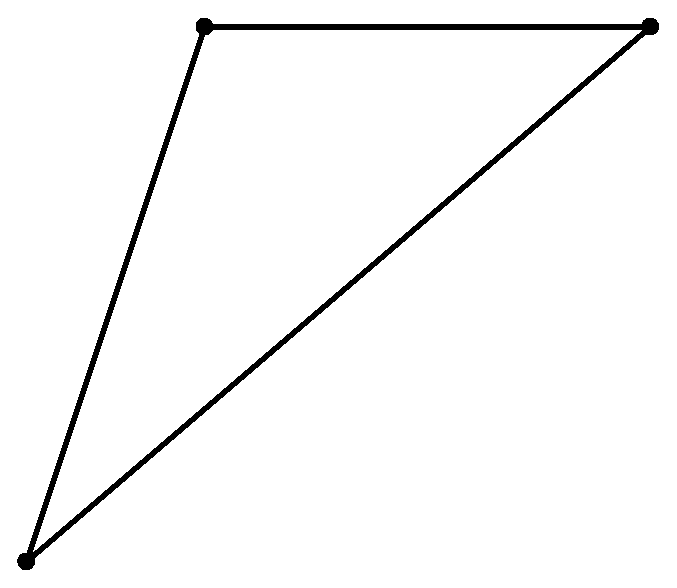
\includegraphics[width=0.35\textwidth]{sketch_triangle}}
    \vspace{0.2in}
    \subfloat[Reference Triangle.]
      {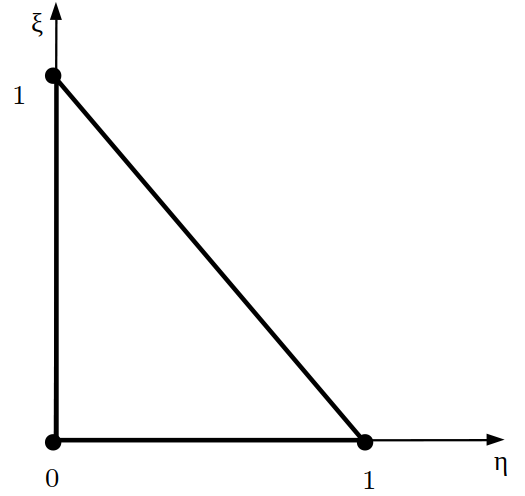
\includegraphics[width=0.35\textwidth]{Tref}}
    %\caption{Description of Triangle Elements.}
    \label{fig:triangle_elements}
  \end{figure}
\end{frame}

\begin{frame}{Wedge Elements}
  \begin{columns}
    \begin{column}{0.5\textwidth}
      \vspace*{\fill}
      \begin{figure}
        \centering
        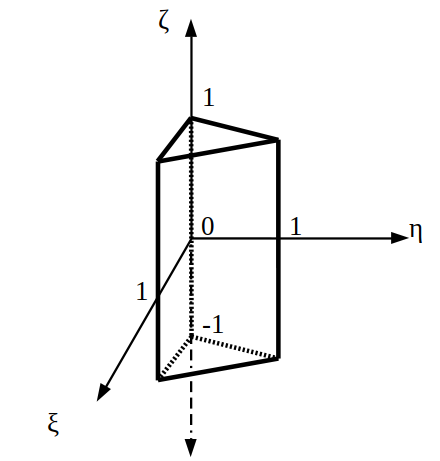
\includegraphics[width=0.8\textwidth]{Wref}
        \caption{Description of Reference Wedge.}
        \label{fig:Wref}
      \end{figure}
      \vspace*{\fill}
    \end{column}
    \begin{column}{0.5\textwidth}
      \begin{figure}
        \centering
        \subfloat[General Wedge Element.]
          {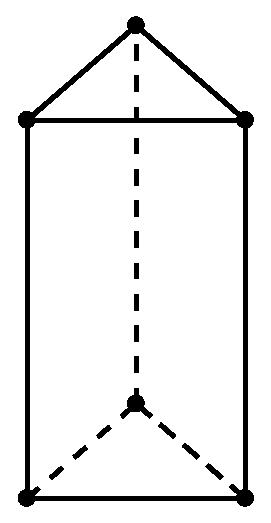
\includegraphics[width=0.4\textwidth]{wedge_sketch}}
        \hspace{0.1\textwidth}
        \subfloat[Distorted Wedge Element.]
          {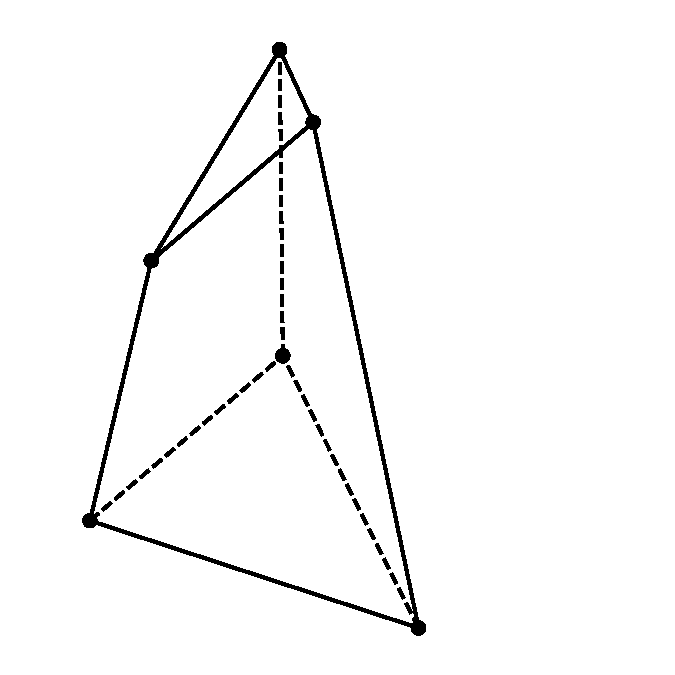
\includegraphics[width=0.4\textwidth]{wedge_stretch}}
        %\caption{Description of Wedge Elements.}
        \label{fig:sketch_wedge}
      \end{figure}
    \end{column}
  \end{columns}
\end{frame}

\begin{frame}{Integration}
  Integrals of interest:
  \begin{align}
    &\int_{\Omega_e} \grad \basis_i(\vr) \cdot \grad \basis_j(\vr) 
      \;d\vr \\
    &\int_{\Omega_e} \basis_i(\vr) \basis_j(\vr) \;d\vr \\
    &\int_{\Omega_e} \basis_i(\vr) \;d\vr \\
    &\int_{\partial \Omega_e} \basis_i(\vr) \basis_j(\vr) \;ds &
  \end{align}

  Options for integration:
  \begin{enumerate}
    \item Analytic.
    \item Numeric (quadrature).
  \end{enumerate}
\end{frame}

\begin{frame}{Quadrature Integration}
  General form with weights $\{w_i\}$ and coordinates $\{\vx_i\}$.
  \begin{equation}
    \label{eq:quadrature}
    \int_{\Omega} f(\vx) \;d\Omega \approx \sum_{i=1}^{N} w_i f(\vx_i)
  \end{equation}
  For integration of a general element using a quadrature centered on a
  reference element, the Jacobian is used.
  \begin{equation}
    \int_{\Omega} f(\vx) \;d\Omega = 
      \int_{\Omega_{ref}} f(\vx) \lvert \mj \rvert \;d\Omega_{ref} \approx
      \sum_{i=1}^{N} w_i f(\vx_i) \lvert \mj_i \rvert
  \end{equation}

  This work uses two types of quadratures.
  \begin{itemize}
    \item Gaussian.
    \item Triangle (symmetric and open).
  \end{itemize}
\end{frame}

\begin{frame}{Power Iterations}
  \begin{itemize}
    \item FEM used to solve spatial distribution $\phi_g(\vr)$ for a given
      source distribution $q_g(\vr)$.
    \item Power Iteration method used to converge to fundamental eigenmode
      (\keff) and eigenvector ($\phi_g(\vr)$).
  \end{itemize}

  The multigroup neutron diffusion equation can be written.
  \begin{equation}
    \label{eq:gehin_notation}
    \mb(\vPhi,\keff) \vPhi = \frac{1}{\keff} \mm \vPhi
  \end{equation}
  Or as an eigenvalue problem.
  \begin{align}
    \label{eq:gehin_solution}
    \vPhi &= \frac{1}{\keff} \mr \vPhi \\
    \label{eq:gehin_r}
    \mr &= \mb^{-1} \mm.
  \end{align}
\end{frame}

\begin{frame}{Power Iterations}
  Using this notation, the Power Iteration method is defined.
  \begin{align}
    \label{eq:power_iteration_phi}
    \vPhi^{(s+1)} &= \frac{1}{\keff^{(s)}} \mr \vPhi^{(s)} \\
    \label{eq:power_iteration_eigenvalue}
    \keff^{(s+1)} &= \keff^{(s)} \frac{\vw^{T} \vPhi^{(s+1)}}
      {\vw^{T} \vPhi^{(s)}} \qquad s = 1,2,\ldots,\infty
  \end{align}

  The weighting is chosen such that $\vw^{T} \vPhi$ is the total fission neutron
  production rate.
  \begin{equation}
    \vw = \{\nu \Sigma_f \}
  \end{equation}

  Convergence rate is described by the dominance ratio.
  \begin{equation}
    d \equiv \frac{\keffsub{0}}{\keffsub{1}}
  \end{equation}
\end{frame}

\begin{frame}{Power Iterations}
  Iteration continues until both $\keff$ and the fission source converge.
  \begin{align}
    \label{eq:eigenvalue_tol}
    \epsilon_{\keff} &> | \keff^{(s+1)} - \keff^{(s)} | \\
    \label{eq:eigenvector_tol}
    \epsilon_{\vPhi} &> \max_i \left| \frac{\nu\Sigma_{f,i}\vPhi_i^{(s+1)} - 
      \nu\Sigma_{f,i} \vPhi_i^{(s)}}
      {\nu\Sigma_{f,i} \vPhi_i^{(s)}}\right| .
  \end{align}
\end{frame}

\begin{frame}{Calculation of Source with Power Iterations}
  Fission and up-scatter sources must lag the flux solution by one iteration
  whereas down-scatter source is known exactly.
  \begin{equation} 
    \label{eq:multigroup_power_iterations}
    -\grad \cdot (D_g(\vr) \grad \phi_g^{(s+1)}(\vr)) + \Sigma_{r,g}(\vr)
    \phi_g^{(s+1)}(\vr) = q_{fiss,g}^{(s)}(\vr) + q_{up,g}^{(s)}(\vr) +
    q_{down,g}^{(s+1)}(\vr)
  \end{equation}
\end{frame}

\begin{frame}{Matrix Ordering}
  \begin{itemize}
    \item Matrix is reordered to increase computational efficiency and compute
      the same solution.
    \item Nodes are re-indexed such that physically proximate nodes have
      proximate indices.
    \item Improve cache hits.
    \item Reverce Cuthill-McKee (RCM) order is chosen \cite{rcm}.
  \end{itemize}
  \vspace{-0.25in}
  \begin{figure}
    \centering
    \subfloat{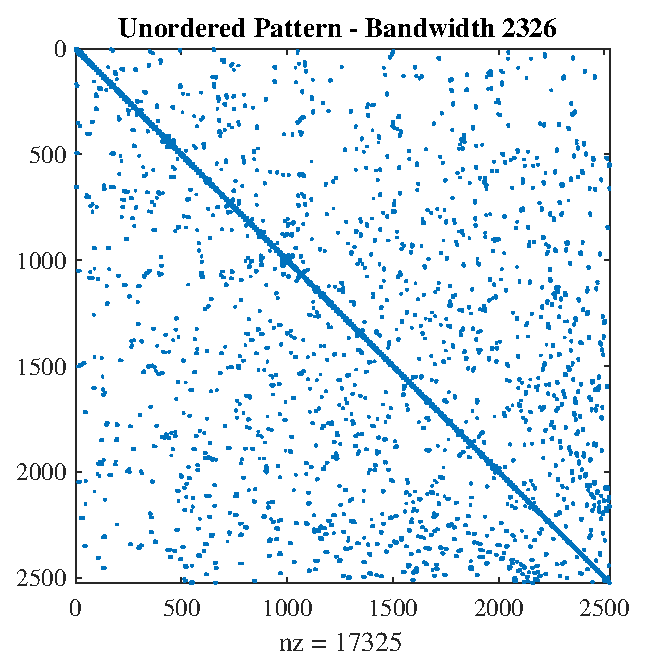
\includegraphics[width=0.4\textwidth]{./figs/uno_pattern}}
    \hspace{0.1in}
    \subfloat{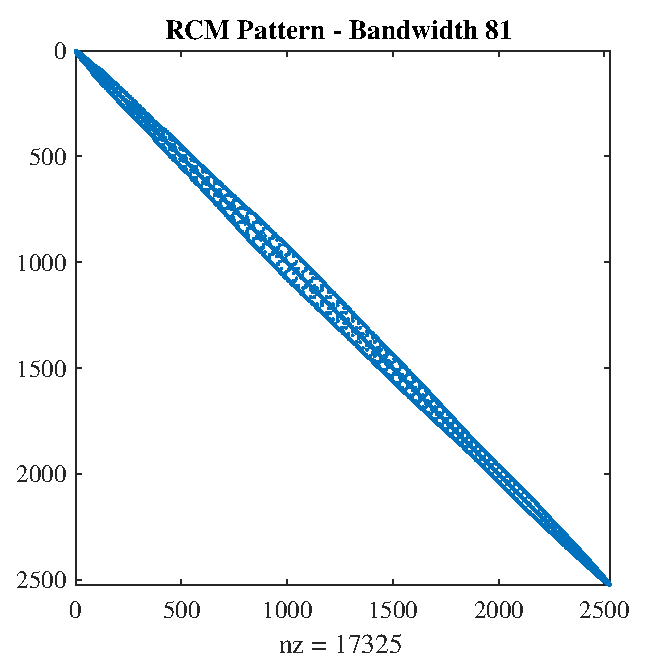
\includegraphics[width=0.4\textwidth]{./figs/rcm_pattern}}
    \label{fig:sparsity_pattern}
  \end{figure}
\end{frame}

\begin{frame}{Memory and Storage}
  \begin{itemize}
    \item Created custom \twotable storage implementation.
    \item Modified reduced row storage.
    \item Designed to minimize storage and optimize matrix vector
      multiplications.
  \end{itemize}
\end{frame}

\begin{frame}{Combined Algorithm}

    \begin{algorithm}[H]
      \caption{\scriptsize General Iteration Scheme}
      \label{algorithm:general}
      \begin{algorithmic}[1]
      \State Read mesh from VTK.
      \State Initialize $\phiavg^{(0)}$.
      \State Order the nodes of the mesh into RCM order.
        \label{state:rcm}
      \State Calculate $\Sigma_s$, $\Sigma_t$, and $\nu \Sigma_f$ for each 
        element.
      \State Calculate finite element matrix $\ma_g$ for each group. Store this. 
        \label{state:fem_matrix}
      \While{Power Iteration}
        \State Update the iteration counter. $s=s+1$
        \State Update $q_{fiss,g}$ and $q_{up,g}$ for all groups from previous 
          data $\phiavg^{(s-1)}$.
        \State Update $\chi$ in each element using previous data.
          \label{state:chi_collapse}
        \For{$g=1,G$}
          \State Update $q_{down,g}$ from current data $\phiavg^{(s)}$
          \State Calculate total effective source in each element.
          \State Update finite element Vector $\vf_g$ with new source.
            \label{state:fem_vector}
          \State Solve $\ma \vu = \vf$ using an iterative technique (Conjugate
            Gradient).
          \State Parse $\vu$ for $\phi$ solution on nodes.
          \State Calculate element-average $\phiavg$.
        \EndFor
        \State Update $\keff$.
        \State Check convergence.
        \State Perform non-linear update if necessary. \label{state:nonlinear}
      \EndWhile
      \end{algorithmic}
    \end{algorithm}

\end{frame}
